\documentclass[12pt]{report}
\usepackage[catalan]{babel}
\usepackage[latin1]{inputenc}   % Permet usar tots els accents i car�ters llatins de forma directa.
\usepackage{enumerate}
\usepackage{amsfonts, amscd, amsmath, amssymb}
\usepackage[pdftex]{graphicx}

\setlength{\textwidth}{16cm}
\setlength{\textheight}{24.5cm}
\setlength{\oddsidemargin}{-0.3cm}
\setlength{\evensidemargin}{0.25cm} \addtolength{\headheight}{\baselineskip}
\addtolength{\topmargin}{-3cm}

\newcommand\Z{\mathbb{Z}}
\newcommand\R{\mathbb{R}}
\newcommand\N{\mathbb{N}}
\newcommand\Q{\mathbb{Q}}
\newcommand\K{\Bbbk}
\newcommand\C{\mathbb{C}}

\newcounter{exctr}
\newenvironment{exemple}
{ \stepcounter{exctr} 
\hspace{0.2cm} 
\textit{Exemple  \arabic{exctr}: }
\it
\begin{quotation}
}{\end{quotation}}

\pagestyle{empty}

\begin{document}

\begin{center}
\textbf{\Large Processament Digital del Senyal.\\ Control 1. Curs 2010-11}
\end{center}

\vskip 1cm
\noindent
\textbf{P1.} Donat el seg�ent sistema:
\[
y[n]={\cal T}(x[n])=\frac{1}{2T+1} \sum_{k=-T}^T x[n-k]
\]

\noindent 
on $T$ �s una constant entera positiva.

\noindent
Es demana:
\begin{enumerate}[a)]
\item Demostrau que �s un sistema LTI.
\item Calculau la resposta impulsional del sistema.
\item Estudiau l'estabilitat i causalitat del sistema a partir de la seva resposta impulsional.
\end{enumerate}

 
\vskip 1cm
\noindent
\textbf{P2.} Considerau el sistema LTI de la figura:

\begin{figure}[htbp]
\begin{center}
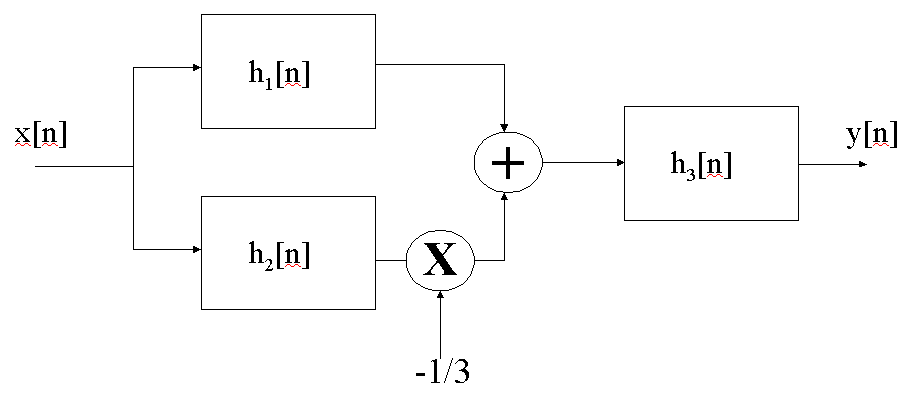
\includegraphics[width=10cm]{figuraP2.png}
\end{center}
\end{figure}
 
\begin{enumerate}[a)]
\item Donau la resposta impulsional del sistema en funci� de $h_1$, $h_2$ i $h_3$
\item Feu el cas particular 
\[
\begin{array}{l}
h_1[n]=\{ 1, 0, \underline{0} \} \\ \\
h_2[n]=n(u[n]-u[n-3]) \\ \\
h_3[n]=(\frac{1}{2})^n u[n-2]
\end{array}
\]
\item Trobau la sortida del sistema quan l'entrada \'es $x[n]=\{ 1, \underline{0}, -1 \}$
\end{enumerate}





\end{document}